\documentclass[a4paper,12pt]{article}

% Paquetes básicos
\usepackage[utf8]{inputenc}
\usepackage[T1]{fontenc}
\usepackage[spanish]{babel}
\usepackage{graphicx}
\usepackage{xcolor}
\usepackage{lipsum}
\usepackage{geometry}
\geometry{top=3cm, bottom=3cm, left=2.5cm, right=2.5cm}

% Paquetes para diseño
\usepackage{titlesec}
\usepackage{fancyhdr}
\usepackage{amsmath}
\usepackage{amssymb}
\usepackage{hyperref}
\usepackage{pdfpages}

% Paquetes para el entorno lstlisting
\usepackage{listings}
\usepackage{inconsolata}

% Paquete para fondo
\usepackage{background}

% Configuración de lstlisting
\lstset{
    language=Python,
    basicstyle=\ttfamily\small,
    keywordstyle=\color{blue}\bfseries,
    stringstyle=\color{teal},
    commentstyle=\color{gray}\itshape,
    numbers=left,
    numberstyle=\tiny\color{gray},
    backgroundcolor=\color{black!5},
    frame=single,
    rulecolor=\color{black!50},
    breaklines=true,
    captionpos=b,
    showstringspaces=false
}

% Configuración de título
\titleformat{\section}{\normalfont\Large\bfseries}{\thesection}{1em}{}

% Información del documento
\title{
    \vspace{-2cm}
    \includegraphics[width=0.3\textwidth]{images/fccee.jpg} \\ % Cambia el logo si es necesario
    \LARGE Ingeniería Informática + ADE\\
    \large Universidad de Granada (UGR)\\[1cm]
}
\author{\textbf{Autor:} Ismael Sallami Moreno}
\date{\textbf{Asignatura:} Dirección y Administración de Empresas}

% Configuración del fondo
\backgroundsetup{
    scale=1,
    color=black,
    opacity=0.2,
    angle=0,
    position=current page.south,
    vshift=0pt,
    hshift=0pt,
    contents={\includegraphics[width=\paperwidth,height=\paperheight,keepaspectratio]{images/granada.jpg}}
}

% Inicio del documento
\begin{document}

% Portada
\maketitle
\thispagestyle{empty}

\begin{center}
    \includegraphics[width=\textwidth,height=0.4\textheight,keepaspectratio]{images/granada.jpg} \\ % Añade tu imagen de fondo
    \vfill
\end{center}

\newpage

% Índice (opcional)
\tableofcontents
\newpage

\section{Tema 1}
\includepdf[pages=-]{../Tema 1.pdf}

\section{Tema 2}
\includepdf[pages=-]{../Tema 2.pdf}

\section{Tema 3}
\includepdf[pages=-]{../Tema 3.pdf}

\section{Tema 4}
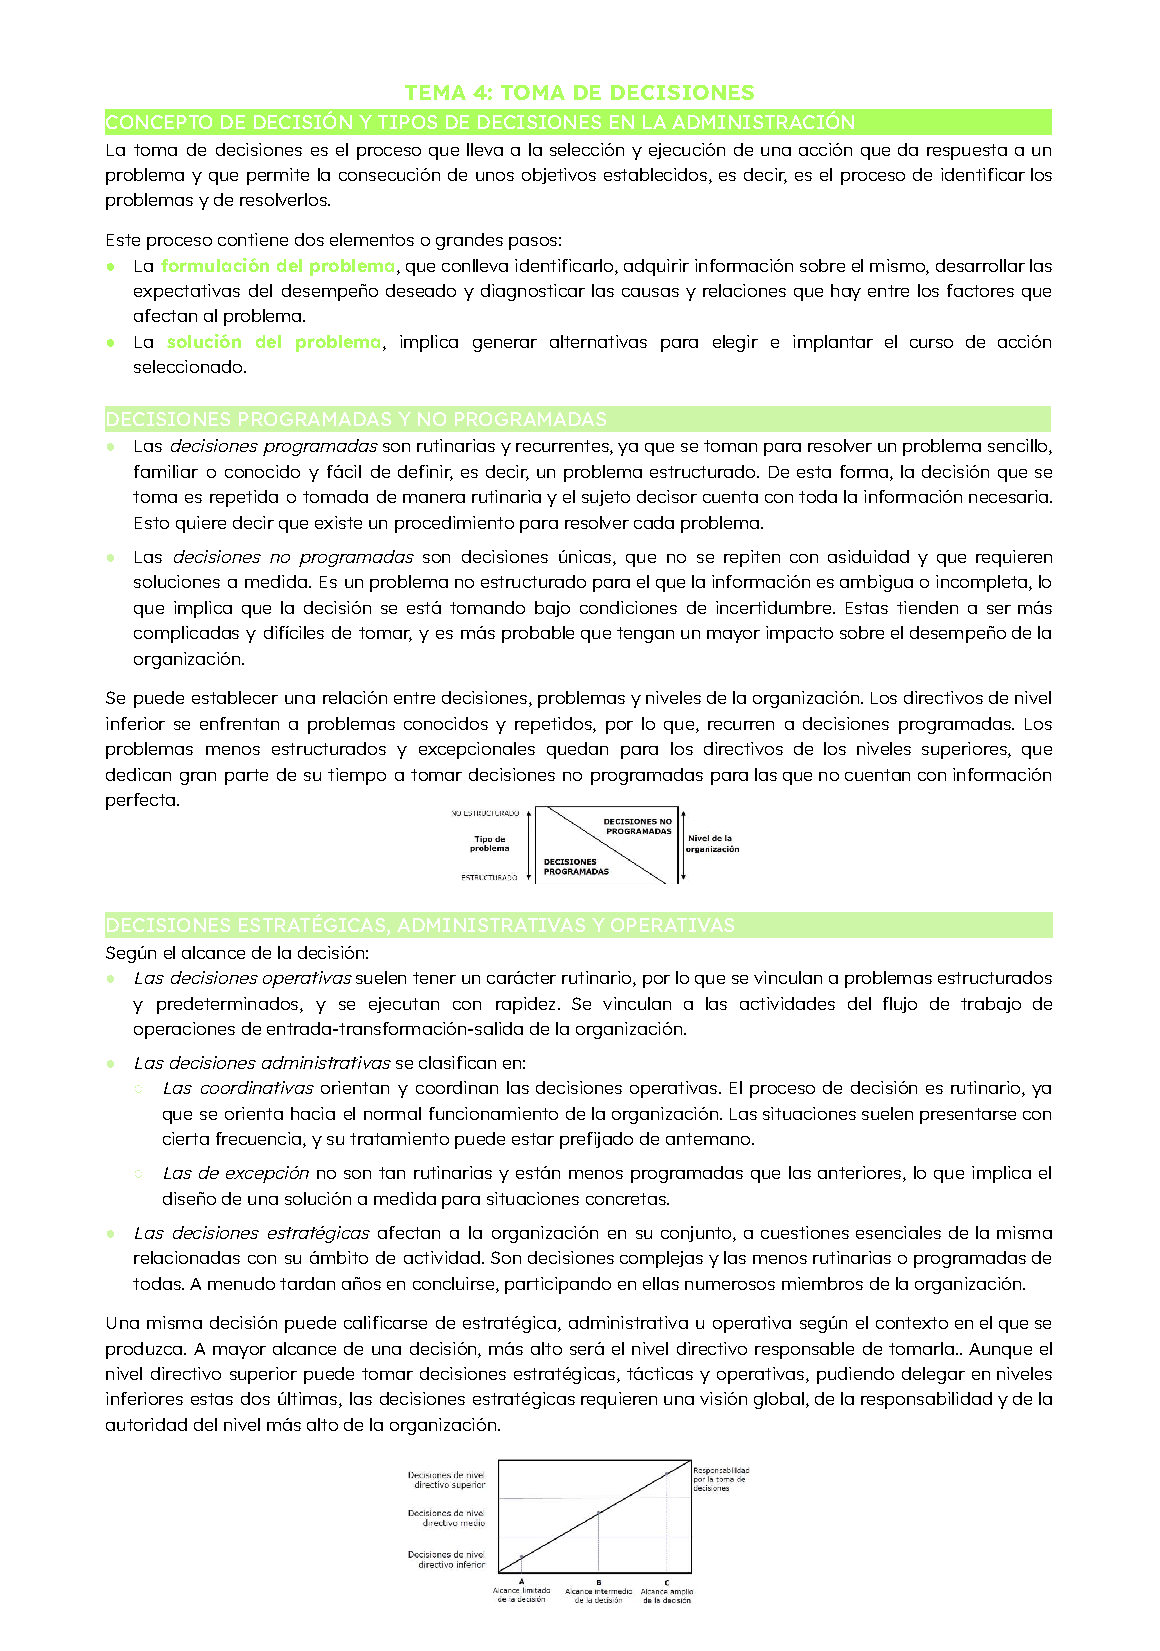
\includepdf[pages=-]{../Tema 4.pdf}

\section{Tema 5}
\includepdf[pages=-]{../Tema 5.pdf}

\section{Tema 6}
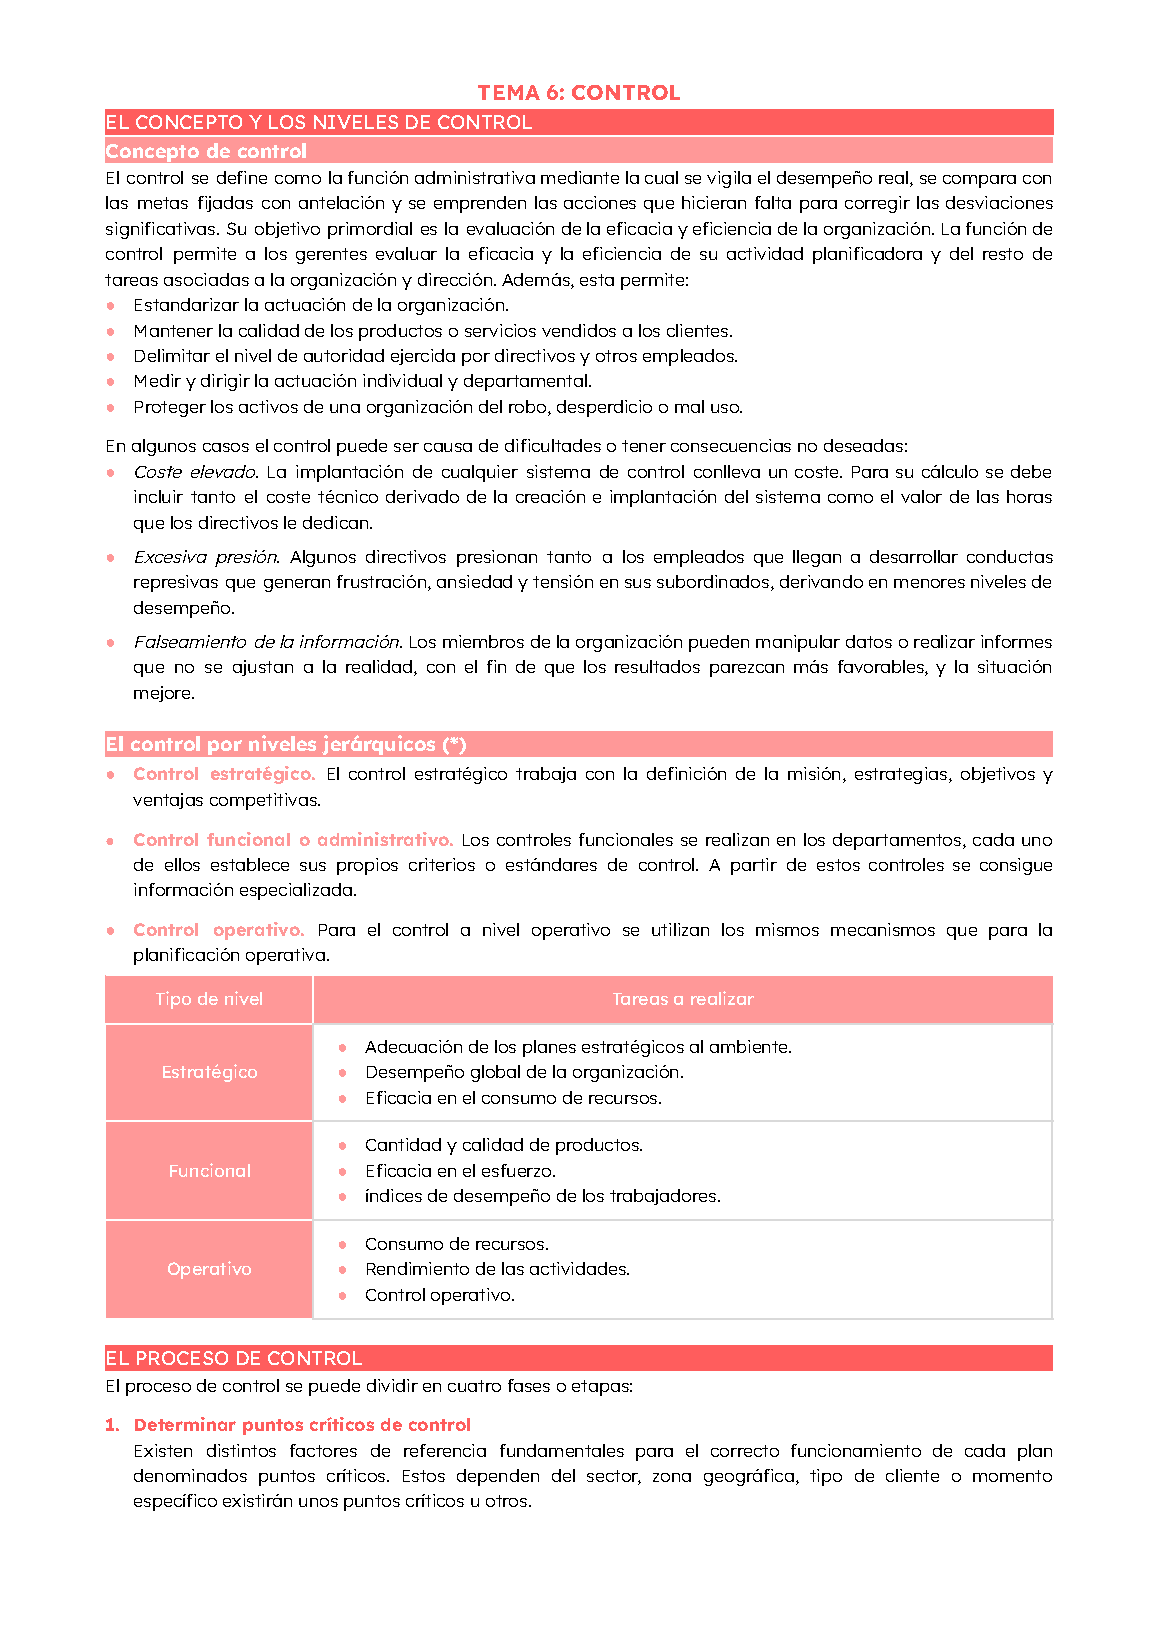
\includepdf[pages=-]{../Tema 6.pdf}

\section{Tema 7}
\includepdf[pages=-]{../Tema 7.pdf}

\section{Tema 8}
\includepdf[pages=-]{../Tema 8.pdf}

\section{Tema 9}
\includepdf[pages=-]{../Tema 9.pdf}

\section{Tema 10}
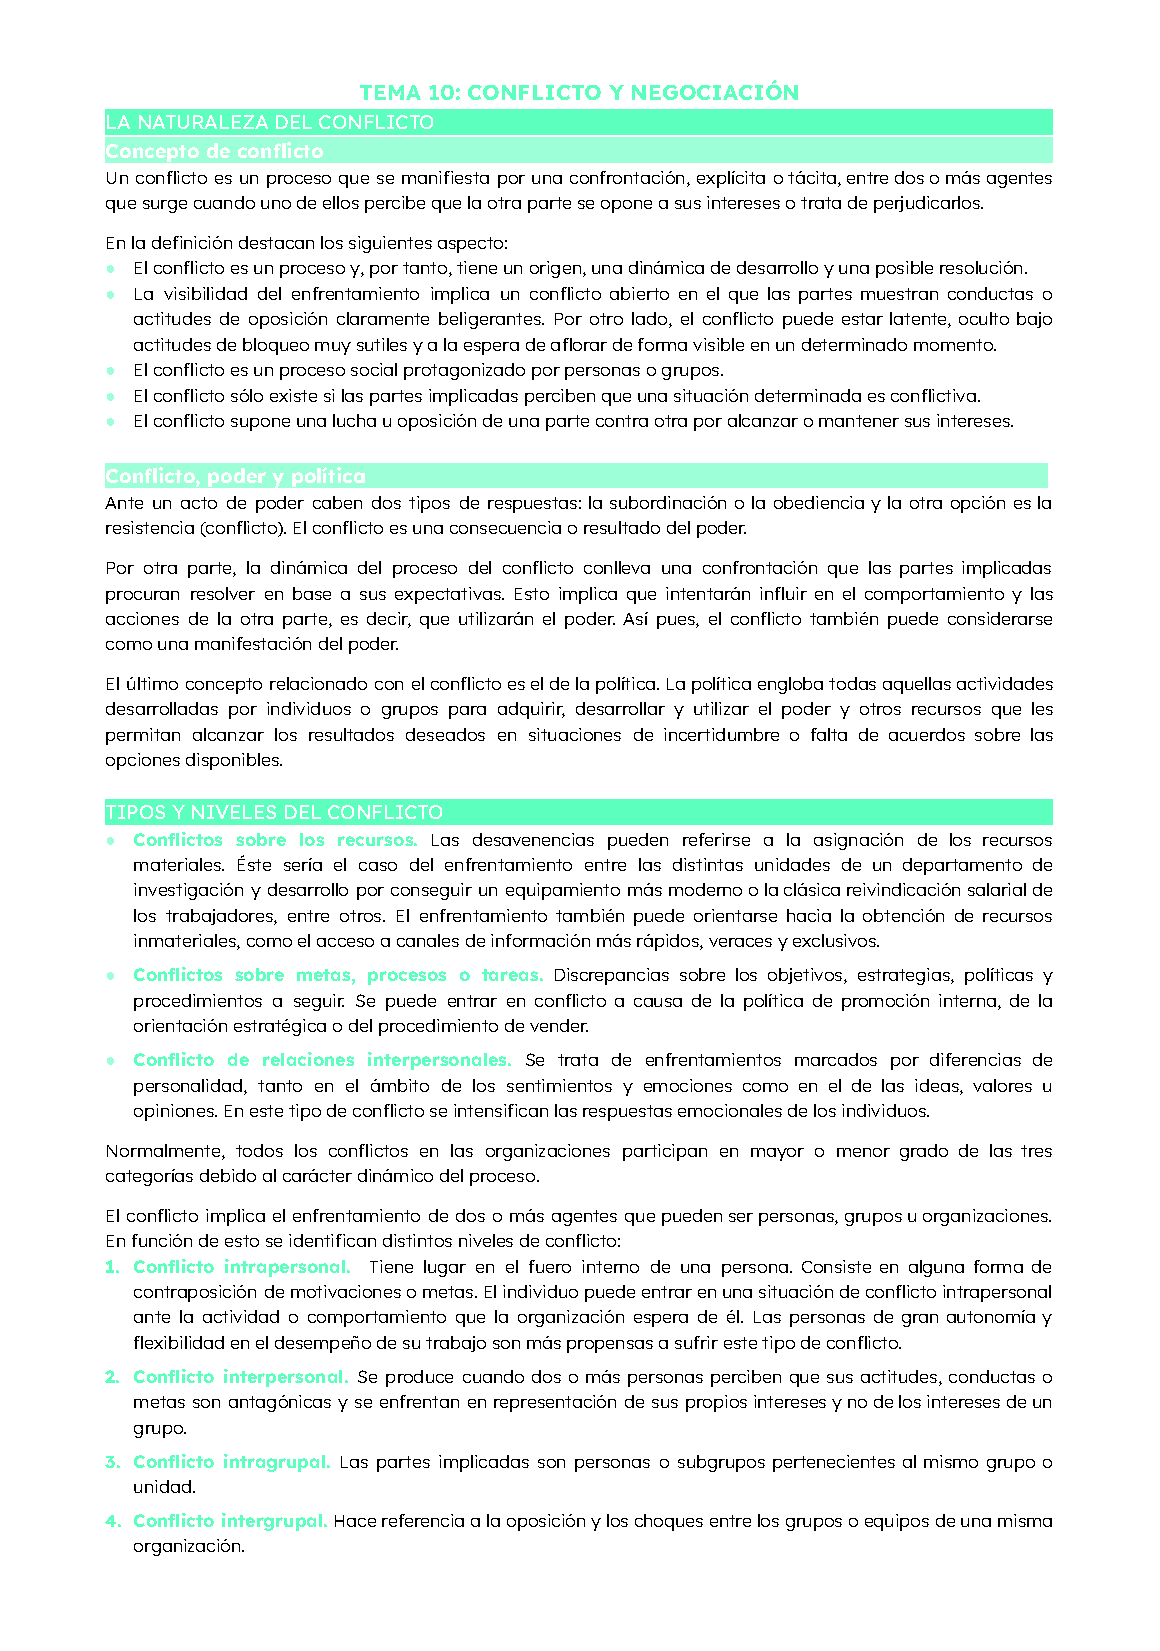
\includepdf[pages=-]{../Tema 10.pdf}



% \section{Tema 1}
% \includepdf[pages=-]{../t1.pdf}

% \section{Tema 2}
% 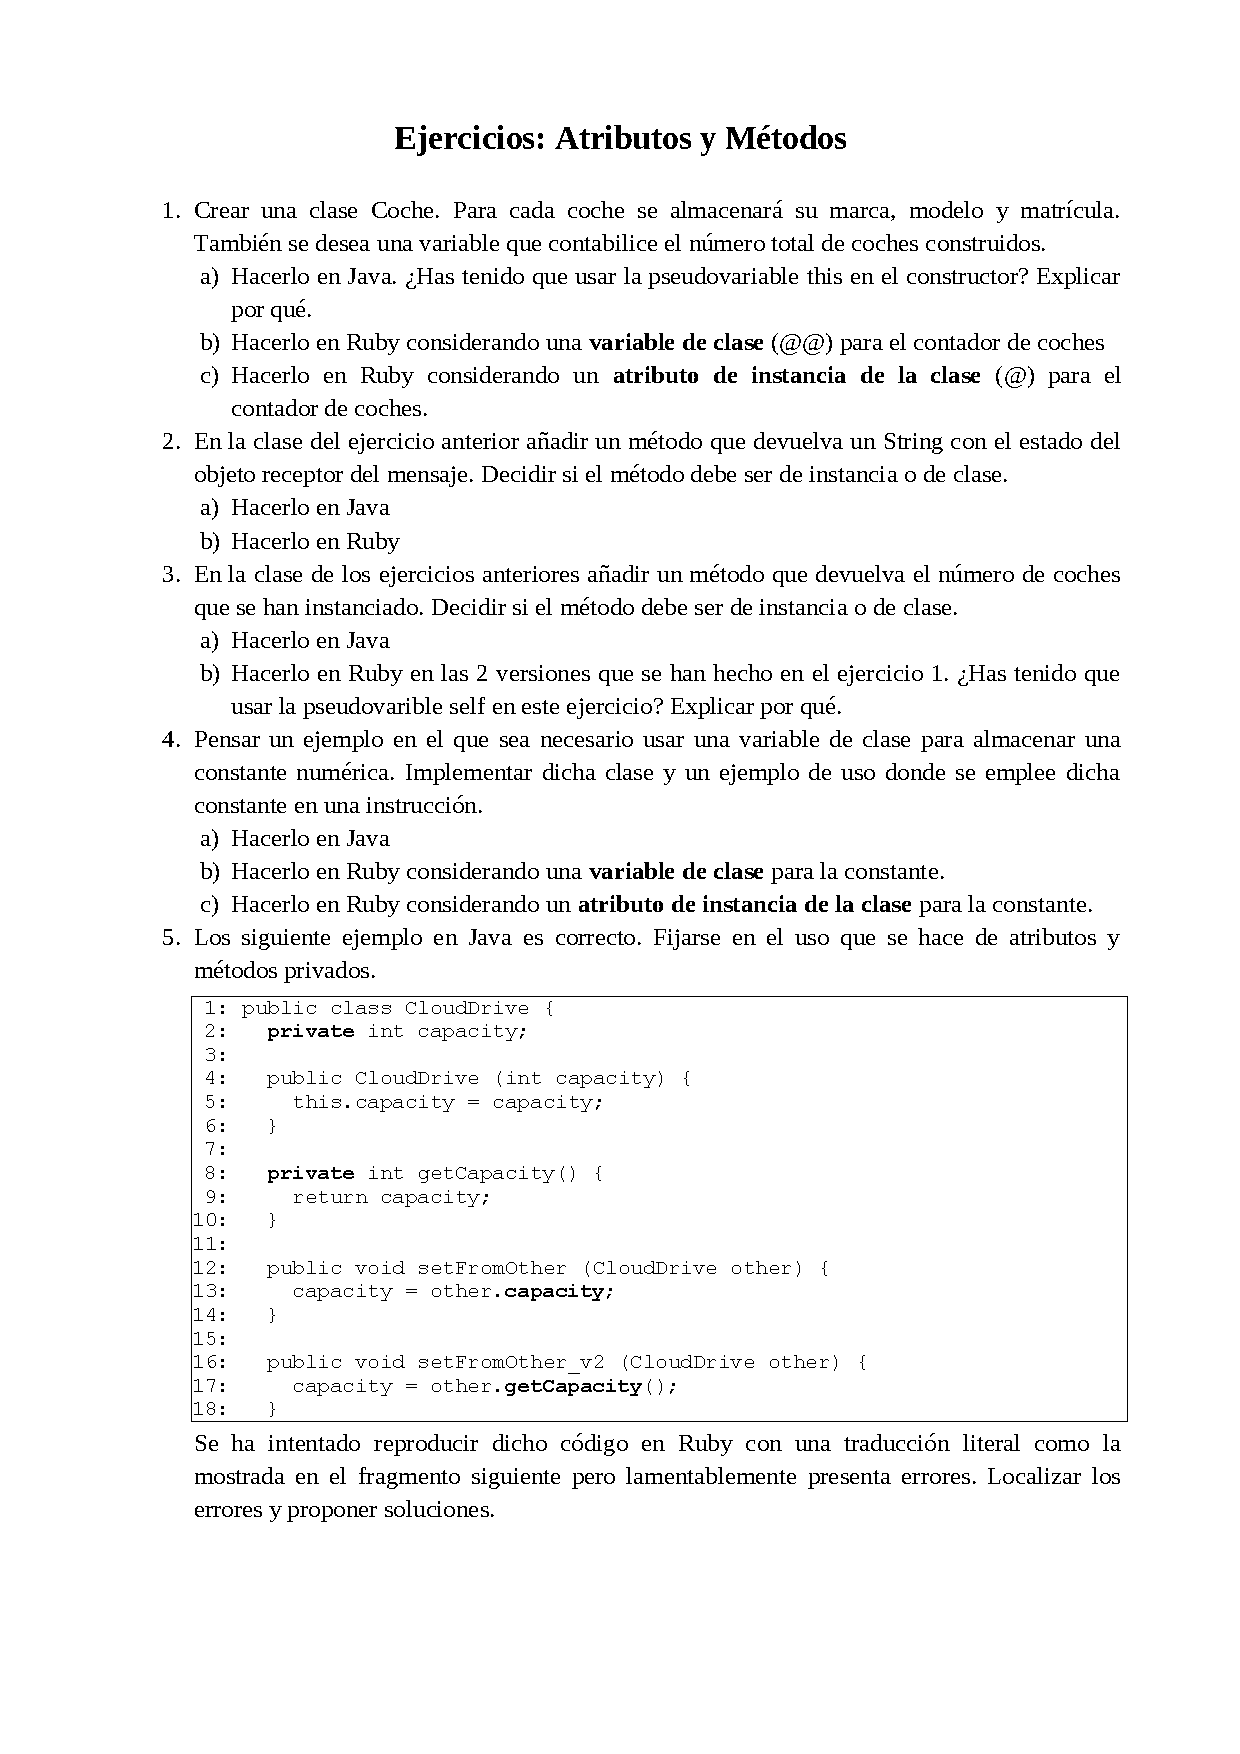
\includepdf[pages=-]{../t2.pdf}

% \section{Tema 3}
% \includepdf[pages=-]{../t3.pdf}

% \section{Tema 4}
% \includepdf[pages=-]{../t4.pdf}

% \section{Tema 5}
% \includepdf[pages=-]{../t5.pdf}

% \section{Tema 6}
% \includepdf[pages=-]{../t6.pdf}

% \section{Tema 7}
% \includepdf[pages=-]{../t7.pdf}

% \section{Tema 8}
% \includepdf[pages={1-7}]{../t8.pdf}

% \section{Tema 9}
% \includepdf[pages=-]{../t9.pdf}

% \section{Tema 10}
% \includepdf[pages=-]{../t10.pdf}

\section{Fuentes}

\begin{itemize}
    \item \url{https://www.wuolah.com}
\end{itemize}


\end{document}
